\documentclass[../main.tex]{subfiles}

\begin{document}

\begin{example}
This is an example where Theorem \ref{Zylev's theorem} fails \par
In $\mathbb H^2$, we can polygons with ideal vertex(vertex at $\infty$)
\begin{center}
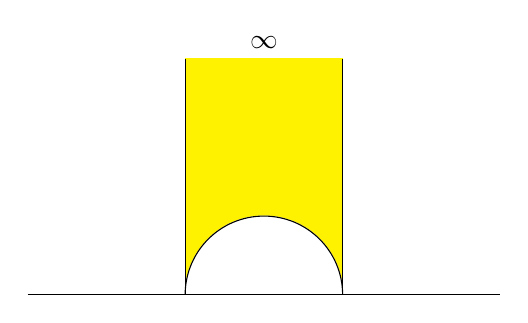
\begin{tikzpicture}
\node[above] at (0,3) {$\infty$};
\clip(-3,0) rectangle (3,3);
\filldraw[yellow] (-1,0) rectangle (1,3);
\filldraw[white] (0,0) circle (1);
\draw(-3,0)--(3,0);
\draw(-1,0)--(-1,3);
\draw(1,0)--(1,3);
\draw (0,0) circle (1);
\end{tikzpicture}
\end{center}
Consider the following situation
\begin{center}
\begin{tikzpicture}
\node[above] at (0,3) {$\infty$};
\clip(-3,0) rectangle (3,3);
\filldraw[yellow] (0,0) circle (2);
\filldraw[white] (-2,0) rectangle (-1,3);
\filldraw[white] (0,0) rectangle (2,3);
\filldraw[white] (-0.5,0) circle (1);
\draw(-4,0)--(4,0);
\draw[name path = left line](-1,0)--(-1,4);
\draw[name path = middle line](0,0)--(0,4);
\draw[name path = right line](1,0)--(1,4);
\draw [dashed] (-0.5,-4)--(-0.5,1);
\draw[name path = large circle] (0,0) circle (2);
\draw[name path = small circle] (-0.5,0) circle (1);
\path[name intersections = {of = small circle and left line, by=a}];
\path[name intersections = {of = small circle and middle line, by=b}];
\path[name intersections = {of = large circle and left line, by=c}];
\path[name intersections = {of = large circle and middle line, by=d}];
\path[name intersections = {of = large circle and right line, by=e}];
\node[above left] at (a) {$a$};
\node[above right] at (b) {$b$};
\node[above left] at (c) {$c$};
\node[above right] at (d) {$d$};
\node[above right] at (e) {$e$};
\end{tikzpicture}
\end{center}
Note here angle $\infty cd$, $\infty ed$, $bac$ and $abd$ are all $60^\circ$ \par
Denote $P_1=cd\infty$, $P_2=de\infty$, $P_3=abdc$, then $P_1\sqcup P_2\sim P_1\sqcup P_3\Rightarrow [P_2]=[P_3]$, but $P_2\not\sim P_3$ since $P_3$ doesn't have ideal vertex
\end{example}

\begin{lemma} $\\$
\textbf{(a) }If $X$ is a $G$ set, then $\mathbb Z[X]$ is a $\mathbb Z[G]$-module($G$-module) \par
\textbf{(b) }If $M$ is an right $R$-module, $N$ is a left $R$-module, then $M\otimes_{R}N$ is an abelian group
\end{lemma}

\begin{proposition}\label{Conversion of the isometry group in scissors congruence}
Treating $\mathbb Z$ as a trivial $G$-module, i.e. $g\cdot 1=1$ \par
\textbf{(a) }If $M$ is a $G$-module, $M\otimes_{\mathbb Z[G]}\mathbb Z=M/\{gm\sim m\}$ \par
\textbf{(b) }If $X$ is a $G$-set, $\mathbb Z[X]\otimes_{\mathbb Z[G]}\mathbb Z=\mathbb Z[X/G]$ \par
\textbf{(c) }If $H\trianglelefteq G$, $\mathbb Z[X]\otimes_{\mathbb Z[G]}\mathbb Z=\mathbb Z[X/H]\otimes_{\mathbb Z[G/H]}\mathbb Z=\mathbb Z[X/G]$ \par
\textbf{(d) }If $H\trianglelefteq G\leq\mathrm{Isom}(X)$, $\mathcal P(X,G)=\mathcal P(X,H)\otimes_{\mathbb Z[G/H]}\mathbb Z$
\end{proposition}

\begin{proof} $\\$
\textbf{(a) }Consider $M\to M\otimes_{\mathbb Z[G]}\mathbb Z$, $m\mapsto m\otimes1$, since $(gm)\otimes1=g(m\otimes1)=m\otimes(g\cdot1)=m\otimes1$, this induce $M/\{gm\sim m\}\to M\otimes_{\mathbb Z[G]}\mathbb Z$, on the other hand, $M/\{gm\sim m\}$ satisfies the universal property \par
\textbf{(b) }$\mathbb Z[X]/\{gx\sim x\}\cong\mathbb Z[X/G]$ \par
\textbf{(c) }$\mathbb Z[X/H]/\{\bar gx\sim x\}\cong\mathbb Z[X/G]$ \par
\textbf{(d) }Let $S$ be the set of simplices in $X$, then $\mathcal P(X,G)=\mathbb Z[S/G]$ is a $G$-module
\end{proof}

\begin{example}
$H=T\trianglelefteq G=\mathrm{Isom}^+(\mathbb R^n)$ is the translation group, $G/H=SO(n)$, $\mathcal P(\mathbb R^n,SO(n))=\mathcal P(\mathbb R^n,T)\otimes_{\mathbb Z[SO(n)]}\mathbb Z$, $\mathcal P(X)=\mathcal P(X,\{1\})\otimes_{\mathbb Z[G]}\mathbb Z$
\end{example}

\begin{theorem} $\\$
\textbf{(a) }$\mathcal P(\mathbb R^1)\cong\mathbb R$ \par
\textbf{(b) }$\mathcal P(S^1)\cong\mathbb R$ \par
\textbf{(c) }$\mathcal P(\mathbb H^1)\cong\mathbb R$ \par
\textbf{(d) }$\mathcal P(\mathbb R^2)\cong\mathbb R$
\end{theorem}

\begin{proof} $\\$
\textbf{(a) }Consider homomorphism $\phi:\mathcal P(\mathbb R^1)\to\mathbb R$, $[I]\mapsto|I|$, sending an interval to its length, this is obviously surjective and injective, thus an isomorphism \par
\textbf{(b) }Consider homomorphism $\phi:\mathcal P(S^1)\to\mathbb R$, $[\theta]\mapsto|\theta|$, sending an arc(angle) to its length, this is obviously surjective and injective, thus an isomorphism \par
\textbf{(c) }$\mathbb R^1\xrightarrow{\exp}\mathbb H^1=\{y|y>0\}$ is an isomorphism \par
\textbf{(d) }Consider homomorphism $\phi:\mathcal P(\mathbb R^2)\to\mathbb R$, $[P]\mapsto|P|$, sending a polygon to its area, according to Theorem \ref{P,Q s.c. <=> P,Q have same area}, this is injective, this is clearly surjective, thus an isomorphism
\end{proof}

\begin{lemma}\label{Scissors congruence group is two divisible}
$\mathcal P(X)$ is $2$ divisible
\end{lemma}

\begin{proof}
Consider the following decomposition about "inscribed sphere center"
\begin{center}
\begin{tikzpicture}[scale=2]
\def\x{1.2038204};
\def\y{0.7440019};
\def\xx{0.53836486};
\def\yy{1.07672972};
\def\xxx{1.7299092};
\def\yyy{1.2700908};
\coordinate (a) at (0,0); \node[left] at (a) {$A$};
\coordinate (b) at (3,0); \node[right] at (b) {$B$};
\coordinate (c) at (1,2); \node[above] at (c) {$C$};
\coordinate (o) at (\x,\y); \node[below right] at ($(o)-(0.05,0)$) {$O$};
\coordinate (d) at (\x,0); \node[below] at (d) {$D$};
\coordinate (e) at (\xx,\yy); \node[above left] at (e) {$E$};
\coordinate (f) at (\xxx,\yyy); \node[above right] at (f) {$F$};
\draw (a)--(b)--(c)--cycle;
\draw (o)--(d);
\draw (o)--(e);
\draw (o)--(f);
\draw (o)--(a);
\draw (o)--(b);
\draw (o)--(c);
\end{tikzpicture}
\end{center}
Denote $P=ABC$, $P_1=AOD$, $Q_1=AOE$, $P_2=BOD$, $Q_2=BOF$, $P_3=COE$, $Q_3=COF$, then we have $[P]=[P_1]+[P_2]+[P_3]+[Q_1]+[Q_2]+[Q_3]=2([P_1]+[P_2]+[P_3])$, hence $\mathcal P(S^2)$ is $2$ divisible, i.e. $\mathcal P(S^2)=2\mathcal P(S^2)$
\end{proof}

\begin{theorem}
$\mathcal P(S^2)\cong\mathbb R$
\end{theorem}

\begin{proof}
Consider homomorphism $\phi:\mathcal P(S^1)\to\mathbb R$, $[\theta]\mapsto|\theta|$, $\psi:\mathcal P(S^2)\to\mathbb R$, $[P]\mapsto|P|$ and $\Sigma:\mathcal P(S^1)\to\mathcal P(S^2)$ defined as follow: suppose $S^1\hookrightarrow S^2$ as equator, $N,S$ are the north and south poles, $\Sigma$ maps arc $AB\subseteq S^1$ to $ABN$ which is clearly injective
\begin{center}
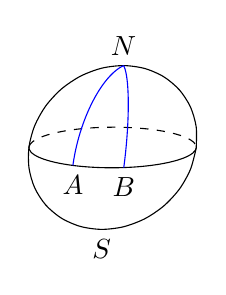
\begin{tikzpicture}
\draw[rotate around z=-5, rotate around x=-8, rotate around y=18] plot[domain=0:180, smooth] ({cos(\x)},{0},{sin(\x)});
\draw[rotate around z=-5, rotate around x=-8, rotate around y=18, dashed] plot[domain=-180:0, smooth] ({cos(\x)},{0},{sin(\x)});
\draw[rotate around z=-5, rotate around x=-8, rotate around y=18] plot[domain=0:360, smooth] ({cos(\x)},{sin(\x)},{0});
\draw[rotate around z=-5, rotate around x=-8, rotate around y=28, blue] plot[domain=0:90, smooth] ({0},{cos(\x)},{sin(\x)});
\draw[rotate around z=-5, rotate around x=-8, rotate around y=-8, blue] plot[domain=0:90, smooth] ({0},{cos(\x)},{sin(\x)});
\node[rotate around z=-5, rotate around x=-8, rotate around y=18, above] at (0,1,0) {$N$};
\node[rotate around z=-5, rotate around x=-8, rotate around y=18, below] at (0,-1,0) {$S$};
\node[rotate around z=-5, rotate around x=-8, rotate around y=-8, below] at (0,0,1) {$A$};
\node[rotate around z=-5, rotate around x=-8, rotate around y=28, below] at (0,0,1) {$B$};
\end{tikzpicture}
\end{center}
Then the following diagram commutes
\begin{center}
\begin{tikzcd}
\mathcal P(S^1) \arrow[dr,"\phi"'] \arrow[r,"\Sigma"] & \mathcal P(S^2) \arrow[d,"\psi"] \\
&\mathbb R
\end{tikzcd}
\end{center}
According to the following picture, $[NBC]+[SBC]=[XYN]+[XYS]=2[XYN]\in\Sigma\mathcal P(S^1)$
\begin{center}
\begin{tikzpicture}[scale=2]
\def\xangle{-19};
\def\yangle{18};
\def\zangle{-5};
\draw[rotate around z=\zangle, rotate around x=\xangle, rotate around y=\yangle] plot[domain=0:180, smooth] ({cos(\x)},{0},{sin(\x)});
\draw[rotate around z=\zangle, rotate around x=\xangle, rotate around y=\yangle, dashed] plot[domain=-180:0, smooth] ({cos(\x)},{0},{sin(\x)});
\draw[rotate around z=\zangle, rotate around x=\xangle, rotate around y=\yangle] plot[domain=0:360, smooth] ({cos(\x)},{sin(\x)},{0});
\draw[rotate around z=\zangle, rotate around x=\xangle, rotate around y={\yangle+10}, blue, name path=circle 1] plot[domain=0:180, smooth] ({0},{cos(\x)},{sin(\x)});
\draw[rotate around z=\zangle, rotate around x=\xangle, rotate around y={\yangle-20}, blue, name path=circle 2] plot[domain=0:180, smooth] ({0},{cos(\x)},{sin(\x)});
\path[rotate around z=\zangle-30, rotate around x=\xangle+30, rotate around y=\yangle, purple, name path=circle 3] plot[domain=0:360, smooth] ({0},{cos(\x)},{sin(\x)});
\path[name intersections = {of = circle 1 and circle 3, by=a}];
\node[right] at (a) {$C$};
\path[name intersections = {of = circle 2 and circle 3, by=b}];
\node[left] at (b) {$B$};
\draw[rotate around z=\zangle-30, rotate around x=\xangle+30, rotate around y=\yangle, purple, name path=circle 3] plot[domain=-165:-83, smooth] ({0},{cos(\x)},{sin(\x)});
\node[rotate around z=\zangle, rotate around x=\xangle, rotate around y=\yangle, above] at (0,1,0) {$N$};
\node[rotate around z=\zangle, rotate around x=\xangle, rotate around y=\yangle, below] at (0,-1,0) {$S$};
\node[rotate around z=\zangle, rotate around x=\xangle, rotate around y={\yangle-20}, below left] at (0,0,1) {$X$};
\node[rotate around z=\zangle, rotate around x=\xangle, rotate around y={\yangle+10}, below right] at (0,0,1) {$Y$};
\end{tikzpicture}
\end{center}
Denote $\overline A$ to be the antipodal point of $A$ and $G=\mathcal P(S^2)/\Sigma\mathcal P(S^1)$, then $[ABC]=-[\overline ABC]$ in $G$, Then 
\begin{align*}
0&=([ABC]+[\overline ABC])+([\overline A\overline BC]+[\overline A\overline B\overline C]) \\
&=[ABC]+([\overline ABC]+[\overline A\overline BC])+[\overline A\overline B\overline C] \\
&=[ABC]+[\overline A\overline B\overline C] \\
&=2[ABC]
\end{align*}
In $G$, thus every element in $G$ is of $2$ torsion, i.e. $2G=0$, by Lemma \ref{Scissors congruence group is two divisible}, $G=2G=0$, $\Sigma$ is an isomorphism
\begin{center}
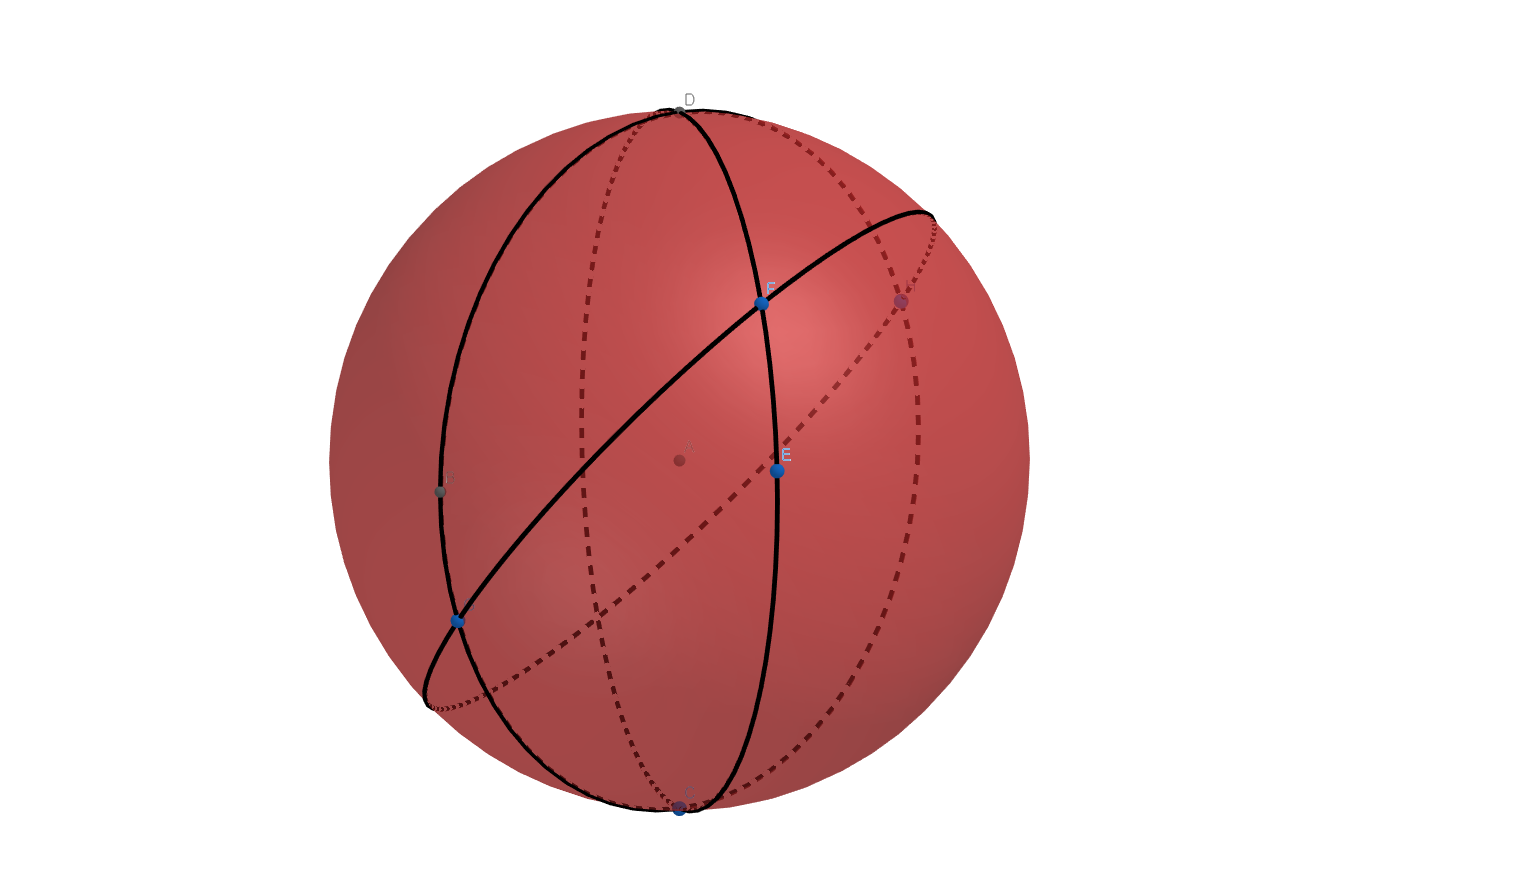
\includegraphics[scale=0.2]{Pictures/Sphere_scissors_congruence.png}
\end{center}
\end{proof}

\end{document}